\documentclass{beamer}
\usepackage[utf8]{inputenc}
\usepackage{graphicx, epsfig}
\usepackage{amsmath,mathrsfs,amsfonts,amssymb}
\usepackage{floatflt}
\usepackage{epic,ecltree}
\usepackage{mathtext}
\usepackage{fancybox}
\usepackage{fancyhdr}
\usepackage{multirow}
\usepackage{enumerate}
\usepackage{epstopdf}
\usepackage{multicol}
\usepackage{algorithm}
\usepackage[noend]{algorithmic}
\usepackage{tikz}
\usepackage{blindtext}
\usetheme{default}%{Singapore}%{Warsaw}%{Warsaw}%{Darmstadt}
\usecolortheme{default}

\setbeamerfont{title}{size=\Huge}
\setbeamertemplate{footline}[page number]{}

\setbeamertemplate{section in toc}[sections numbered]


\makeatletter
\newcommand\HUGE{\@setfontsize\Huge{35}{40}}
\makeatother    

\setbeamerfont{title}{size=\HUGE}
\beamertemplatenavigationsymbolsempty

% latin bold lower
\newcommand{\ba}{\mathbf{a}} 
\newcommand{\bc}{\mathbf{c}} 
\newcommand{\be}{\mathbf{e}} 
\newcommand{\bh}{\mathbf{h}} 
\newcommand{\bp}{\mathbf{p}} 
\newcommand{\bt}{\mathbf{t}} 
\newcommand{\bs}{\mathbf{s}} 
\newcommand{\bu}{\mathbf{u}} 
\newcommand{\bv}{\mathbf{v}} 
\newcommand{\bw}{\mathbf{w}} 
\newcommand{\bx}{\mathbf{x}} 
\newcommand{\by}{\mathbf{y}} 
\newcommand{\bz}{\mathbf{z}} 

% latin bold upper
\newcommand{\bA}{\mathbf{A}} 
\newcommand{\bB}{\mathbf{B}} 
\newcommand{\bC}{\mathbf{C}} 
\newcommand{\bI}{\mathbf{I}} 
\newcommand{\bL}{\mathbf{L}} 
\newcommand{\bM}{\mathbf{M}} 
\newcommand{\bQ}{\mathbf{Q}} 
\newcommand{\bT}{\mathbf{T}} 
\newcommand{\bU}{\mathbf{U}} 
\newcommand{\bV}{\mathbf{V}} 
\newcommand{\bW}{\mathbf{W}} 
\newcommand{\bX}{\mathbf{X}} 
\newcommand{\bY}{\mathbf{Y}} 
\newcommand{\bZ}{\mathbf{Z}} 

% latin cal upper
\newcommand{\cG}{\mathcal{G}} 
\newcommand{\cL}{\mathcal{L}} 
\newcommand{\cN}{\mathcal{N}} 
\newcommand{\cS}{\mathcal{S}} 
\newcommand{\cT}{\mathcal{T}} 
\newcommand{\cW}{\mathcal{W}} 
\newcommand{\cX}{\mathcal{X}} 
\newcommand{\cZ}{\mathcal{Z}} 

% latin bb upper
\newcommand{\bbE}{\mathbb{E}} 
\newcommand{\bbI}{\mathbb{I}} 
\newcommand{\bbP}{\mathbb{P}} 
\newcommand{\bbR}{\mathbb{R}} 

% greek bold lower
\newcommand{\bepsilon}{\boldsymbol{\epsilon}} 
\newcommand{\btheta}{\boldsymbol{\theta}} 
\newcommand{\blambda}{\boldsymbol{\lambda}} 
\newcommand{\bpi}{\boldsymbol{\pi}} 
\newcommand{\bmu}{\boldsymbol{\mu}} 
\newcommand{\bsigma}{\boldsymbol{\sigma}} 
\newcommand{\bphi}{\boldsymbol{\phi}} 

% greek bold upper
\newcommand{\bSigma}{\boldsymbol{\Sigma}} 

\DeclareMathOperator*{\argmin}{arg\,min}
\DeclareMathOperator*{\argmax}{arg\,max}

\newcommand{\createdgmtitle}[1]{\title[\hbox to 56mm{Deep Generative Models  \hfill\insertframenumber\,/\,\inserttotalframenumber}]
	{Deep Generative Models \\ {\Huge Lecture #1}}
	\author{Roman Isachenko}
	\institute{
\includegraphics[width=0.5cm]{../utils/ozonmasterslogo} \large{Ozon Masters}}
	\date{Spring, 2022}
}

\newcommand\myfootnote[1]{%
  \tikz[remember picture,overlay]
  \draw (current page.south west) +(1in + \oddsidemargin,0.5em)
  node[anchor=south west,inner sep=0pt]{\parbox{\textwidth}{%
      \rlap{\rule{10em}{0.4pt}}\raggedright\scriptsize \textit{#1}}};}

\newcommand\myfootnotewithlink[2]{%
  \tikz[remember picture,overlay]
  \draw (current page.south west) +(1in + \oddsidemargin,0.5em)
  node[anchor=south west,inner sep=0pt]{\parbox{\textwidth}{%
      \rlap{\rule{10em}{0.4pt}}\raggedright\scriptsize\href{#1}{\textit{#2}}}};}
      
\AtBeginSection[]
{
	\begin{frame}{Outline}
		\tableofcontents[currentsection,subsectionstyle=hide]
	\end{frame}
}
\AtBeginSubsection[]{
	\begin{frame}{Outline}
		\tableofcontents[currentsection,currentsubsection]
	\end{frame}
}
\createdgmtitle{13}
%--------------------------------------------------------------------------------
\begin{document}
%--------------------------------------------------------------------------------
\begin{frame}[noframenumbering,plain]
%\thispagestyle{empty}
\titlepage
\end{frame}
%=======
\begin{frame}{Outline}
	\tableofcontents
\end{frame}
%=======
\section{Neural ODE: finish}
%=======
\begin{frame}{Neural ODE}
	\begin{block}{Adjoint functions}
		\vspace{-0.3cm}
		\[
			\ba_{\bz}(t) = \frac{\partial L(\by)}{\partial \bz(t)}; \quad \ba_{\btheta}(t) = \frac{\partial L(\by)}{\partial \btheta(t)}.
		\]
		\vspace{-0.6cm}
	\end{block}
	\begin{block}{Theorem (Pontryagin)}
	\vspace{-0.6cm}
	\[
	     \frac{d \ba_{\bz}(t)}{dt} = - \ba_{\bz}(t)^T \cdot \frac{\partial f(\bz(t), \btheta)}{\partial \bz}; \quad \frac{d \ba_{\btheta}(t)}{dt} = - \ba_{\bz}(t)^T \cdot \frac{\partial f(\bz(t), \btheta)}{\partial \btheta}.
	\]
	Do we know any initilal condition?
	\end{block}
	\begin{block}{Solution for adjoint function}
		\vspace{-0.8cm}
		\begin{align*}
			 \frac{\partial L}{\partial \btheta(t_0)} &= \ba_{\btheta}(t_0) =  - \int_{t_1}^{t_0} \ba_{\bz}(t)^T \frac{\partial f(\bz(t), \btheta)}{\partial \btheta(t)} dt + 0\\
			 \frac{\partial L}{\partial \bz(t_0)} &= \ba_{\bz}(t_0) =  - \int_{t_1}^{t_0} \ba_{\bz}(t)^T \frac{\partial f(\bz(t), \btheta)}{\partial \bz(t)} dt + \frac{\partial L}{\partial \bz(t_1)}\\
		\end{align*}
		\vspace{-1.5cm}
	\end{block}
	\textbf{Note:} These equations are solved back in time.
	\myfootnotewithlink{https://arxiv.org/abs/1806.07366}{Chen R. T. Q. et al. Neural Ordinary Differential Equations, 2018}   
\end{frame}
%=======
\begin{frame}{Neural ODE}
	\vspace{-0.2cm}
	\begin{block}{Forward pass}
		\vspace{-0.5cm}
		\[
			\bz(t_1) = \int^{t_1}_{t_0} f(\bz(t), \btheta) d t  + \bz_0 \quad \Rightarrow \quad \text{ODE Solver}
		\]
		\vspace{-0.6cm}
	\end{block}
	\begin{block}{Backward pass}
		\vspace{-0.8cm}
		\begin{equation*}
			\left.
				{\footnotesize 
				\begin{aligned}
					\frac{\partial L}{\partial \btheta(t_0)} &= \ba_{\btheta}(t_0) =  - \int_{t_1}^{t_0} \ba_{\bz}(t)^T \frac{\partial f(\bz(t), \btheta)}{\partial \btheta(t)} dt + 0 \\
					\frac{\partial L}{\partial \bz(t_0)} &= \ba_{\bz}(t_0) =  - \int_{t_1}^{t_0} \ba_{\bz}(t)^T \frac{\partial f(\bz(t), \btheta)}{\partial \bz(t)} dt + \frac{\partial L}{\partial \bz(t_1)} \\
					\bz(t_0) &= - \int^{t_0}_{t_1} f(\bz(t), \btheta) d t  + \bz_1.
				\end{aligned}
				}
			\right\rbrace
			 \Rightarrow
			\text{ODE Solver}
		\end{equation*}
		\vspace{-0.4cm} 
	\end{block}
	\textbf{Note:} These scary formulas are the standard backprop in the discrete case.
	\begin{figure}
		\centering
		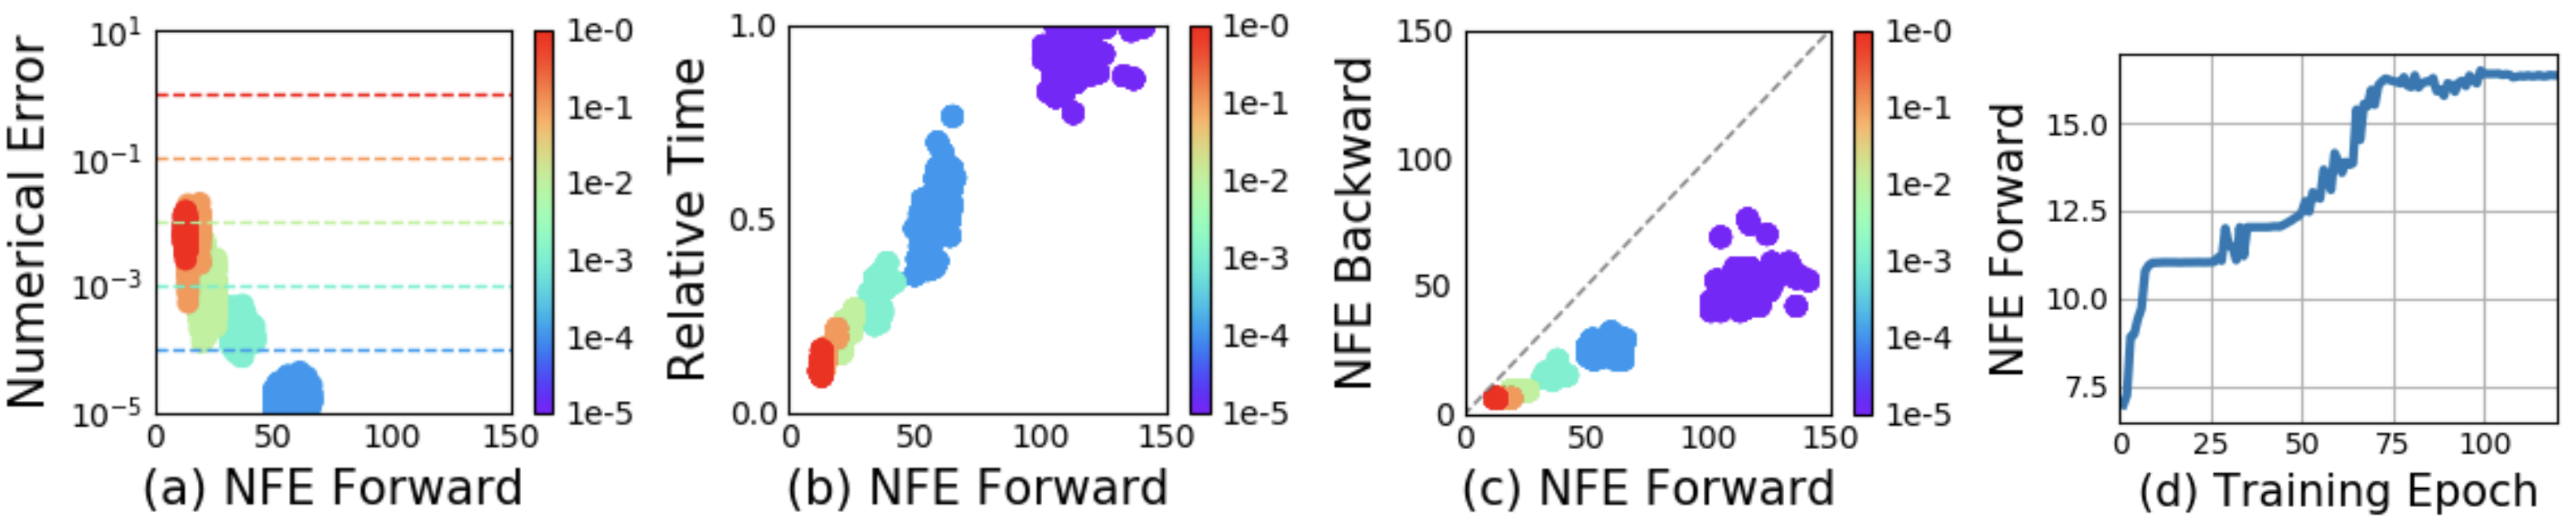
\includegraphics[width=\linewidth]{figs/neural_ode}
	\end{figure}
	\myfootnotewithlink{https://arxiv.org/abs/1806.07366}{Chen R. T. Q. et al. Neural Ordinary Differential Equations, 2018}   
\end{frame}
%=======
\section{Continuous-in-time normalizing flows}
%=======
\begin{frame}{Continuous Normalizing Flows}
	\begin{block}{Discrete Normalizing Flows}
		\vspace{-0.8cm}
		  \[
		  \bz_{t+1} = f(\bz_t, \btheta); \quad \log p(\bz_{t+1}) = \log p(\bz_{t}) - \log \left| \det \frac{\partial f(\bz_t, \btheta)}{\partial \bz_{t}} \right| .
		  \]
		\vspace{-0.7cm}
	\end{block}
	\begin{block}{Continuous-in-time dynamic transformation}
		\vspace{-0.2cm}
		\[
			\frac{d\bz(t)}{dt} = f(\bz(t), \btheta).
		\]
		\vspace{-0.4cm}
	\end{block}
	Assume that function $f$ is uniformly Lipschitz continuous in $\bz$ and continuous in $t$. From Picard’s existence theorem, it follows that the above ODE has a \textbf{unique solution}.
	\begin{block}{Forward and inverse transforms}
		\vspace{-0.7cm}
		\begin{align*}
			\bx &= \bz(t_1) = \bz(t_0) + \int_{t_0}^{t_1} f(\bz(t), \btheta) dt \\
			\bz &= \bz(t_0) = \bz(t_1) + \int_{t_1}^{t_0} f(\bz(t), \btheta) dt \\
		\end{align*}
	\end{block}
	\myfootnotewithlink{https://arxiv.org/abs/1912.02762}{Papamakarios G. et al. Normalizing flows for probabilistic modeling and inference, 2019}   
\end{frame}
%=======
\begin{frame}{Continuous Normalizing Flows}
	To train this flow we have to get the way to calculate the density~$p(\bz(t))$.
	\begin{block}{Theorem (special case of Kolmogorov-Fokker-Planck)}
		if function $f$ is uniformly Lipschitz continuous in $\bz$ and continuous in $t$, then
		\vspace{-0.3cm}
		\[
			\frac{d \log p(\bz(t))}{d t} = - \text{trace} \left( \frac{\partial f (\bz(t), \btheta)}{\partial \bz(t)} \right).
		\]
		\vspace{-0.5cm}
	\end{block}
	\textbf{Note:} Unlike discrete-in-time flows, the function $f$ does not need to be bijective, because uniqueness guarantees that the entire transformation is automatically bijective.
	\begin{block}{Density evaluation}
		\vspace{-0.4cm}
		\[
			\log p(\bx | \btheta) = \log p(\bz) - \int_{t_0}^{t_1} \text{trace}  \left( \frac{\partial f (\bz(t), \btheta)}{\partial \bz(t)} \right) dt.
		\]
		\textbf{Adjoint} method is used to integral evaluation.
	\end{block}
	\myfootnotewithlink{https://arxiv.org/abs/1806.07366}{Chen R. T. Q. et al. Neural Ordinary Differential Equations, 2018}   
\end{frame}
%=======
\begin{frame}{Continuous Normalizing Flows}
	\vspace{-0.6cm}
	\begin{block}{Forward transform + log-density}
		\vspace{-0.8cm}
		\[
			\begin{bmatrix}
				\bx \\
				\log p(\bx | \btheta)
			\end{bmatrix}
			= 
			\begin{bmatrix}
				\bz \\
				\log p(\bz)
			\end{bmatrix} + 
			\int_{t_0}^{t_1} 
			\begin{bmatrix}
				f(\bz(t), \btheta) \\
				- \text{trace} \left( \frac{\partial f(\bz(t), \btheta)}{\partial \bz(t)} \right) 
			\end{bmatrix} dt.
		\]
		\vspace{-0.6cm}
	\end{block}
	\begin{itemize}
		\item Discrete-in-time normalizing flows need invertible $f$. It costs $O(d^3)$ to get determinant of Jacobian.
		\item Continuous-in-time flows require only smoothness of $f$. It costs $O(d^2)$ to get trace of Jacobian.
	\end{itemize}
	\vspace{-0.5cm}
	\begin{minipage}[t]{0.4\columnwidth}
		\begin{figure}
			\centering
			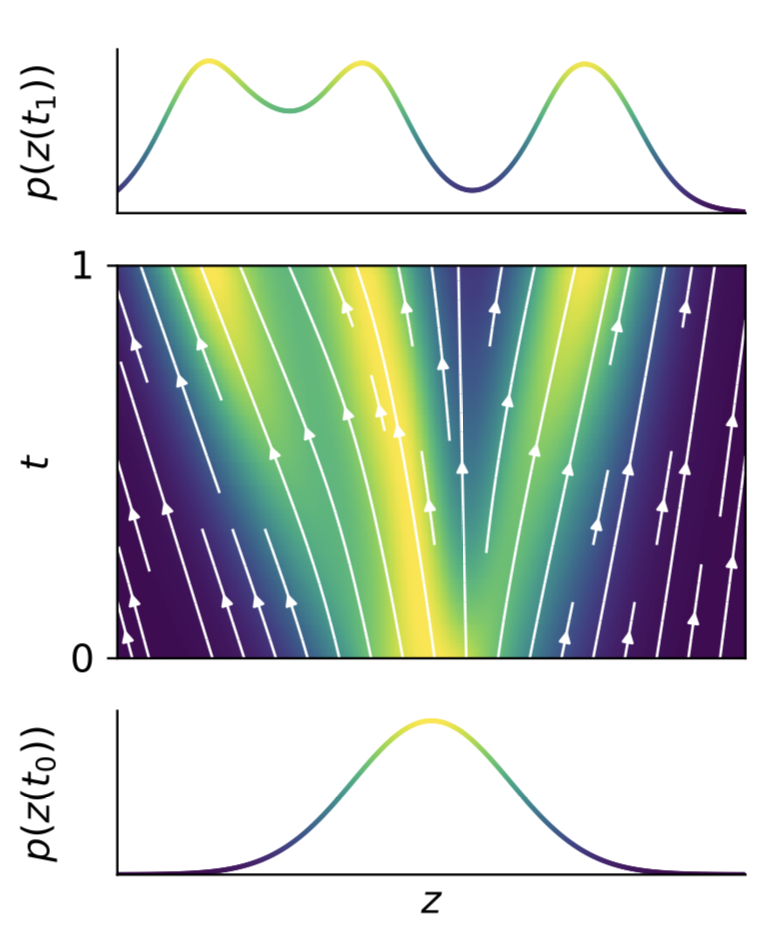
\includegraphics[width=0.75\linewidth]{figs/cnf_flow.png}
		\end{figure}
	\end{minipage}%
	\begin{minipage}[t]{0.6\columnwidth}
		\begin{figure}
			  \centering
			  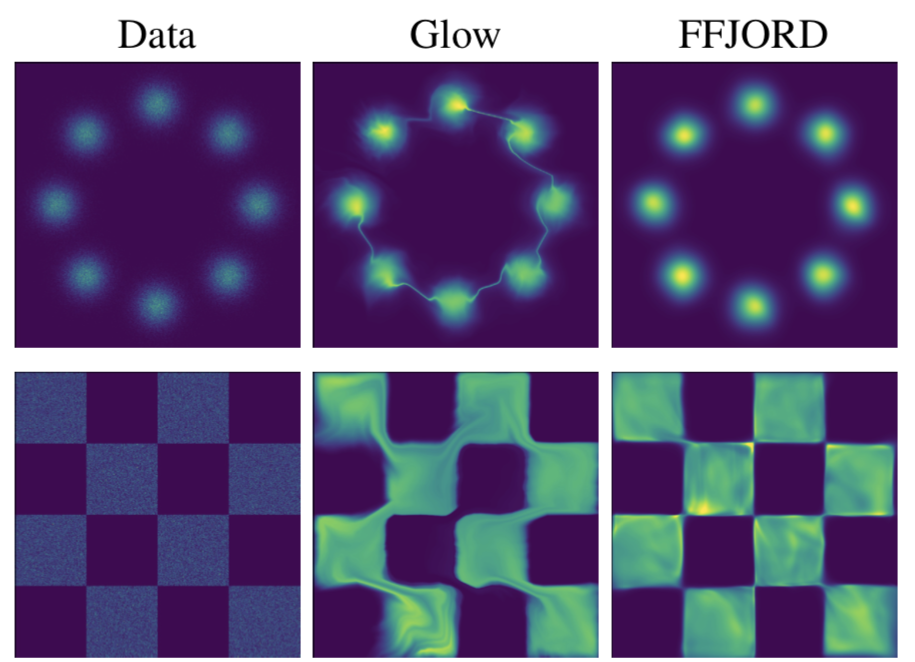
\includegraphics[width=0.8\linewidth]{figs/ffjord.png}
		\end{figure}
	\end{minipage}
	\myfootnotewithlink{https://arxiv.org/abs/1810.01367}{Grathwohl W. et al. FFJORD: Free-form Continuous Dynamics for Scalable Reversible Generative Models, 2018} 
\end{frame}
%=======
\section{Stochastic differential equations basics (SDE)}
%=======
\begin{frame}{Stochastic differential equation (SDE)}
	Let define stochastic process $\bx(t)$ with initial condition $bx(0) \sim p_0(\bx)$:
	\[
		d\bx = \mathbf{f}(\bx, t) dt + g(t) d \bw
	\]
	\begin{itemize}
	\item $\bw(t)$ is the standard Wiener process (Brownian motion)
	\[		
		\bw(t) - \bw(s) \sim \cN(0, t - s), \quad d \bw = \epsilon \cdot \sqrt{dt}, \, \text{where } \epsilon \sim \cN(0, 1).
	\]
	 \item $\mathbf{f}(\bx, t)$ is the \textbf{drift} function of $\bx(t)$.
	 \item $g(t)$ is the \textbf{diffusion} coefficient of $\bx(t)$.
	 \item If $g(t) = 0$ we get standard ODE.
	\end{itemize}
\end{frame}
%=======
\begin{frame}{Stochastic differential equation (SDE)}
	\[
		d\bx = \mathbf{f}(\bx, t) dt + g(t) d \bw
	\]
 	How to get distribution $p(\bx | t)$ for $\bx(t)$?
	\begin{block}{Theorem (Kolmogorov-Fokker-Planck)}
		Evolution of the distribution $p(\bx | t)$ is given by the folliwing ODE:
		\[
			\frac{\partial p(\bx|t)}{\partial t} = - \frac{\partial}{\partial \bx} \bigl( \mathbf{f}(\bx, t) p(\bx)\bigr) + \frac{1}{2} g^2(t) \frac{\partial^2 p(\bx | t)}{\partial \bx^2} 
		\]
	\end{block}
\end{frame}
%=======
\begin{frame}{Stochastic differential equation (SDE)}
	\begin{block}{Langevin SDE}
		Let consider special case of SDE with $g(t) = 1$ and $\mathbf{f}(\bx, t) = \frac{1}{2} \frac{\partial}{\partial \bx} \log p(\bx | t)$.
		\[
			d \bx = \frac{1}{2} \frac{\partial}{\partial \bx} \log p(\bx | t) d t + d \bw
		\]
		Let apply KFP theorem.
		\begin{multline*}
			\frac{\partial p(\bx|t)}{\partial t} =  - \frac{\partial}{\partial \bx}\left( p(\bx | t) \frac{1}{2} \frac{\partial}{\partial \bx} \log p(\bx | t) \right)  + \frac{1}{2} \frac{\partial^2 p(\bx | t)}{\partial \bx^2} = \\
			= - \frac{\partial}{\partial \bx}\left( \frac{1}{2} \frac{\partial}{\partial \bx} p(\bx | t) \right)  + \frac{1}{2} \frac{\partial^2 p(\bx | t)}{\partial \bx^2} = 0
		\end{multline*}
		The density is $p(\bx | t) = \text{const}$.
	\end{block}
	\begin{block}{Langevin dynamic}
		Let discretize the Langevin SDE
		\[
			\bx_{t + 1} = \bx_t + \eta \frac{1}{2} \frac{\partial}{\partial \bx} \log p(\bx | t) + \sqrt{\eta} \cdot \epsilon, \quad \epsilon \sim \cN{0, 1}.
		\]
	\end{block}
\end{frame}
%=======
\begin{frame}{Stochastic differential equation (SDE)}
	\begin{block}{Langevin dynamic}
		Let discretize the Langevin SDE
		\[
			\bx_{t + 1} = \bx_t + \eta \frac{1}{2} \frac{\partial}{\partial \bx} \log p(\bx | t) + \sqrt{\eta} \cdot \epsilon, \quad \epsilon \sim \cN{0, 1}.
		\]
	\end{block}
\end{frame}
%=======
\begin{frame}{Summary}
	\begin{itemize}
		\item Adjoint method generalizes backpropagation procedure and allows to train Neural ODE solving ODE for adjoint function back in time.
		\vfill
		\item Fokker-Planck theorem allows to construct continuous-in-time normalizing flow with less functional restrictions.
		\vfill
		\item FFJORD model makes such kind of flows scalable.
		\vfill
	\end{itemize}
\end{frame}
\end{document} 